\documentclass[oneside, final, 14pt]{extreport}
\usepackage[utf8]{inputenc}
\usepackage[russian]{babel}
\usepackage{vmargin}
\setpapersize{A4}
\setmarginsrb{2cm}{1cm}{1cm}{1cm}{0pt}{0mm}{0pt}{13mm}
\usepackage{indentfirst}
\usepackage{amsmath}
\usepackage{graphicx}
\usepackage{wrapfig}
\sloppy

\begin{document}
  
\setcounter{chapter}{1}
\chapter{Восприятие звука человеком, элементы психофизиологической акустики}
{\itshape Акустика} (от греч. "<akustikos">~--- слуховой) в широком смысле~--- это область физики, изучающая возникновение, распространение и взаимодействие с веществом звуковых волн от самых низких частот до самых высоких; в узком смысле~--- учение о звуке. Основными разделами акустики являются:
\begin{itemize}
\item общая акустика, 
\item прикладная акустика 
\item психофизиологическая акустика.
\end{itemize}

{\itshape Психофизиологическая акустика}~--- это наука, изучающая психологические и физиологические особенности восприятия звука человеком. Основными задачами психофизиологической акустики являются: 
\begin{itemize}
\item исследование влияния звука на человека;
\item исследование процесса получения и обработки звуковой информации мозгом человека;
\item выработка правил, норм и рекомендаций по нейтрализации вредного влияния звука на человека при нахождении его в звуковой среде, а также при использовании различной звуковой аппаратуры и приборов.
\end{itemize} 

На данной лекции, опираясь на науку "<Психофизиологическая акустика">, мы рассмотрим комплекс вопросов, связанных с восприятием звука человеком, в частности~--- как и в каком частотном диапазоне человек воспринимает звук, каковы особенности и возможности слухового аппарата человека, а также психофизиологические акустические параметры звука и т.д. 

\section{Слуховой аппарат человека}
В анатомии ухо человека принято делить на три части (рис. \ref{pic-ear-01}): 
\begin{itemize}
\item наружное ухо;
\item среднее ухо;
\item внутреннее ухо.
\end{itemize}

\begin{figure}[h]
\centering
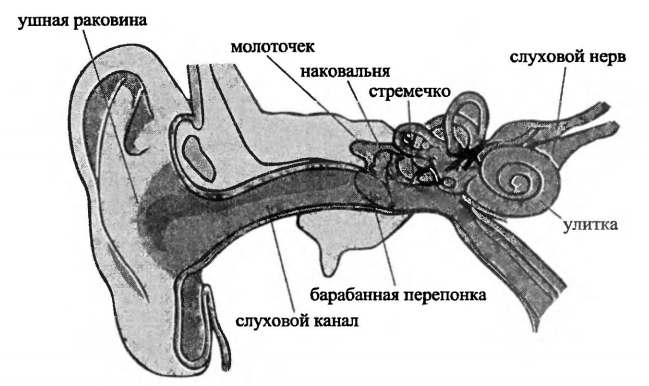
\includegraphics{pic-ear-01}
\caption{Анатомия уха человека}
\label{pic-ear-01}
\end{figure}

К наружному уху относятся {\itshape ушная раковина}, помогающая сконцентрировать звуковые колебания, и {\itshape наружный слуховой канал}. Звуковая волна, попадая в ушную раковину, проходит дальше по слуховому каналу (его длина составляет около
3 см, а диаметр~--- около 0,5 см) и попадает в среднее ухо, где ударяется о {\itshape барабанную перепонку}, представляющую собой тонкую полупрозрачную мембрану. Барабанная перепонка преобразует звуковую волну в вибрации, при этом усиливая эффект от слабой звуковой волны и ослабляя от сильной. Эти вибрации передаются по присоединенным к барабанной перепонке {\itshape косточкам} (молоточку, наковальне и стремечку) во внутреннее ухо, представляющее собой завитую трубку с жидкостью диаметром около 0,2 мм и длиной около 4 см. Эта трубка называется улиткой. Внутри улитки находится еще одна мембрана, называемая базилярной мембраной, напоминающая узкую ленту длиной 32 мм, вдоль которой располагаются нервные окончания (более 20 тысяч волокон). Толщина базилярной мембраны в начале улитки и в ее вершине различна. В результате такого строения мембрана резонирует разными своими частями в ответ на звуки разной высоты. Так, звуковые колебания высокой частоты затрагивают нервные окончания, располагающиеся в начале улитки, а колебания низкой частоты~--- нервные окончания в ее вершине. Звуковые колебания воспринимаются нервными окончаниями по двум принципам~--- ударному и частотному.

{\itshape Ударный принцип} заключается в том, что нервные окончания в вершине улитки сами по себе способны передавать мозгу информацию не только о наличии сигнала, но и о частоте колебаний, если эта частота не превышает $400-450$ Гц. Таким
образом, низкочастотные колебания передаются в мозг нервными окончаниями, расположенными в вершине улитки, в виде импульсов определенной частоты. 

Но благодаря примененной Природой хитрости этими нервными окончаниями в мозг передаются колебания с частотами вплоть до $4000$ Гц. Суть хитрости состоит в том, что колебания затрагивают не один нерв, а сразу не♥сколько. При этом затронутые нервные окончания в вершине улитки воспринимают колебания с определенной временной задержкой (ведь окончания расположены вдоль мембраны, а значит, время прихода колебаний на разные участки мембраны различно). Так, проанализировав частоту колебаний на разных участках мембраны, мозг способен различить колебания с частотами приблизительно до 4 кГц.

Более высокочастотные колебания передаются уже в соответствии с {\itshape частотным принципом}, когда колебания различных частот затрагивают нервные окончания в разных участках в начале улитки. При этом мозг уже различает частоту
колебаний не по частоте нервных импульсов, как в предыдущем случае, а лишь по месторасположению затронутых нервных окончаний в улитке. Таким образом, улитку можно сравнить с набором резонаторов, каждый из которых чувствителен к колебаниям звука в некоторой полосе частот.

Итак, основную информацию о звуковых колебаниях мозг получает в области частот до 4 кГц. Этот факт оказывается вполне логичным, если учесть, что все основные жизненно необходимые человеку звуки (голоса людей, животных, шум воды, ветра и пр.) находятся именно в этой спектральной полосе. Частоты выше 4 кГц являются для человека вспомогательными, что подтверждается многими опытами. Например, можно легко убедиться в том, что человек почти не способен разобрать речь и другие природные звуки, если из этих звуков "<удалить"> частоты от 0 до 4 кГц, оставив только более высокие частотные составляющие. Одновременно с этим слышимость частот выше 4 кГц, как дополнение к основным частотам, создает у человека ощущение более качественного звучания. Поэтому принято считать, что низкие частоты "<ответственны"> за разборчивость и ясность аудиоинформации, а высокие частоты~--- за субъективное качество звука.

Слуховой аппарат человека способен различать частотные составляющие звука приблизительно в пределах от 20-30 Гц до 20 кГц (слышимый звук). 

Указанная верхняя граница может колебаться в зависимости от возраста человека и других факторов. Заметим, что речь идет именно о способности слухового аппарата. Частоты ниже 20-30 Гц (инфразвук) человек также способен воспринимать, но только уже не ухом, а всем телом, как вибрации.

Особое место в слуховом аппарате человека занимает базилярная мембрана. Все специфические особенности слуха человека связаны с устройством и механизмом ее работы. Рассмотрим механизм работы базилярной мембраны подробнее.
Как мы уже говорили, базилярная мембрана имеет длину 32 мм и является той частью слуховой системы, которая улавливает звуковые сигналы и передает их в мозг. Для наглядности "<развернем"> эту мембрану и рассмотрим происходящие в ней процессы (рис. \ref{pic-ear-02}).

%\begin{wrapfigure}[11]{r}{0.75\linewidth} 
\begin{figure}
\centering
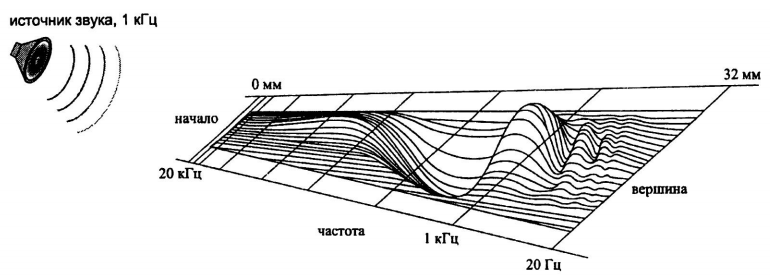
\includegraphics[width=0.75\textwidth]{pic-ear-02}
\caption{Схема базилярной мембраны}
\label{pic-ear-02}
%\end{wrapfigure}
\end{figure}

Ширина и толщина "ленты" мембраны в начале улитки меньше ширины и толщины в конце улитки (в ее вершине). Звуковой сигнал, приходящий со стороны начала улитки, заставляет мембрану резонировать в разных частях. Мембрана устроена так, что высокие частоты вызывают возбуждения в начале мембраны (там мембрана жестче), а низкие частоты~--- в конце (там она мягче). Максимальные колебания мембраны происходят в той ее части, которая соответствует частоте приходящей звуковой волны. Тонкие волокна, расположенные вдоль мембраны и оказавшиеся в резонирующей области, начинают колебаться, возбуждая тем самым нервные окончания, которые передают информацию о колебаниях в мозг. При
этом, конечно, начинает колебаться не какая-то одна точка мембраны, а целый отрезок мембраны (ведь мембрана~--- это своего рода узкая лента типа струны) с центром в точке, соответствующей частоте возбуждения. Так мозг получает и идентифицирует информацию о возмущениях с той или иной частотой. Анализируя информацию о характере возмущений мембраны (месте и времени), мозг, выступая в роли, подобной спектроанализатору, интерпретирует их, как звук той или иной высоты.

В качестве примера на рис. \ref{pic-ear-02} схематично показано воздействие на мембрану сигнала с частотой 1 кГц. Как видно из рисунка, приходящий звуковой сигнал колеблет мембрану на некотором определенном ее участке. Этот эффект похож на принцип действия обыкновенного полосно-пропускающего фильтра с той лишь разницей, что центр полосы пропускания в случае базилярной мембраны будет находиться в точке, соответствующей частоте возбуждающего сигнала (назовем эту частоту центральной частотой). 

Всю мембрану в целом можно представить как набор слуховых полосно-пропускающих фильтров, расположенных в определенном порядке (по частоте убывания от 20 кГц до 20 Гц) с определенной величиной перекрытия, покрывающих всю полосу слышимых частот. При этом физическая ширина (площадь) каждого такого слухового фильтра на мембране тем больше, чем выше его центральная частота, и наоборот. Ширина слухового фильтра, измеренная в герцах, составляет приблизительно 10-20\% от его центральной частоты. Например, ширина фильтра с центральной частотой 13,5 кГц
составляет приблизительно 3,5 кГц. Примечательно, что для частот до 500 Гц ширина слуховых фильтров остается приблизительно постоянной и составляет 100 Гц.

На рис. \ref{pic-ear-03} показан график, отображающий зависимость ширины слуховых
фильтров от их центральной частоты.

\begin{figure}[h]
\centering
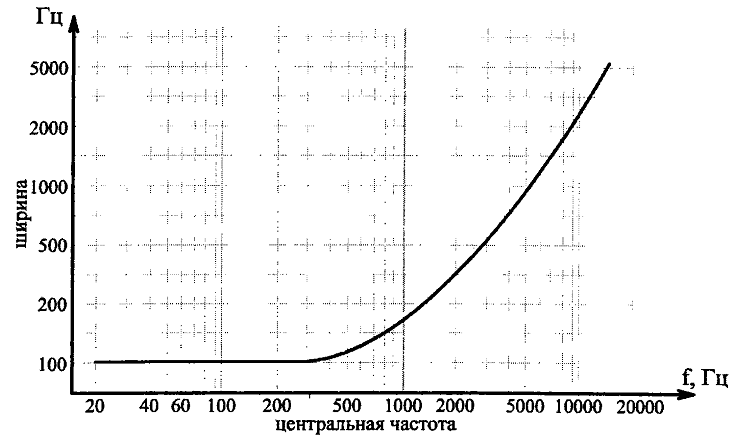
\includegraphics[width=0.9\linewidth]{pic-ear-03}
\caption{Зависимость ширины слуховых фильтров от их центральной частоты}
\label{pic-ear-03}
\end{figure}

На приведенном графике по оси абсцисс откладывается значение центральной частоты, а по оси ординат - ширина соответствующего слухового фильтра.

С наличием описанных слуховых фильтров связывают понятие критической полосы. 

{\itshape Критическая полоса} (называемая также "<полоса разборчивости">) ~--- это минимальная полоса частот, которая возбуждает одну и ту же часть базилярной мембраны. 

В частотном промежутке от 0 до 16 кГц опытным путем были определены 24 критические полосы: 0-100 Гц, 100-200 Гц, 200-300 Гц, 300-400 Гц, 400-510 Гц, 510-630 Гц, 630-770 Гц, 770-920 Гц, 920-1080 Гц, 1080-1270 Гц, 1270-1480 Гц, 1480-1720 Гц, 1720-2000 Гц, 2000-2320 Гц, 2320-2700 Гц, 2700-3150 Гц, 3150-3700 Гц, 3700-4400 Гц, 4400-5300 Гц, 5300-6400 Гц, 6400-7700 Гц, 7700-9500 Гц, 9500-12 000 Гц и 12 000-15 500 Гц.

Звуковой сигнал в пределах одной и той же критической полосы как бы обобщается мозгом, создавая близкие слуховые ощущения. Если же звуковой сигнал переходит из одной критической полосы в другую, то слуховые ощущения в момент перехода заметно изменяются, потому что мозг анализирует информацию, полученную из разных критических полос, раздельно. Это совершенно не значит, что два тона, попавшие в одну критическую полосу, не различимы на слух, просто это значит, что слуховые ощущения внутри одной полосы очень близки, а в разных полосах~--- отличаются существенно (об этом мы еще будем говорить чуть ниже).

Участки базилярной мембраны, соответствующие критическим полосам, имеют
приблизительно равную длину, которая составляет 1,2 мм на полосу. Для удобства
работы с критическими полосами существует специальная единица измерения частоты~--- {\itshape Барк}. В табл. \ref{tab-crit-01} приведены 24 критические полосы и соответствующие им параметры.

\begin{table}[h!]
  \caption{Критические полосы и соответствующие им параметры}
  \begin{center}
  \begin{tabular}{|p{0.10\textwidth}|p{0.20\textwidth}|p{0.20\textwidth}|p{0.20\textwidth}|}
  \hline Номер полосы, Барк & Критическая полоса, Гц & Ширина критической полосы, Гц & Центральная частота критической полосы, Гц \\
  \hline 0 & \centering 0 - 0 & \centering 100 & 50 \\
  \hline 1 & \centering 100 - 200 &\centering 100 & 150 \\
  \hline 2 & \centering 200 - 300 &\centering 100 & 250 \\
  \hline 3 & \centering 300 - 400 &\centering 100 & 350 \\
  \hline 4 & \centering 400 - 510 &\centering 110 & 450 \\
  \hline 5 & \centering 510 - 630 &\centering 120 & 570 \\
  \hline 6 & \centering 630 - 770 &\centering 140 & 700 \\
  \hline 7 & \centering 770 - 920 &\centering 150 & 840 \\
  \hline 8 & \centering 920 - 1080 &\centering 160 & 1000 \\
  \hline 9 & \centering 1080 - 1270 &\centering 190 & 1170 \\
  \hline 10 & \centering 1270 - 1480 &\centering 210 & 1370 \\
  \hline 11 & \centering 1480 - 1720 &\centering 240 & 1600 \\
  \hline 12 & \centering 1720 - 2000 &\centering 280 & 1850 \\
  \hline 13 & \centering 2000 - 2310 &\centering 320 & 2150 \\
  \hline 14 & \centering 2320 - 2700 &\centering 380 & 2500 \\
  \hline 15 & \centering 2700 - 3150 &\centering 450 & 2900 \\
  \hline 16 & \centering 3150 - 3700 &\centering 550 & 3400 \\
  \hline 17 & \centering 3700 - 4400 &\centering 700 & 4000 \\
  \hline 18 & \centering 4400 - 5300 &\centering 900 & 4800 \\
  \hline 19 & \centering 5300 - 6400 &\centering 1100 & 5800 \\
  \hline 20 & \centering 6400 - 7700 &\centering 1300 & 7000 \\
  \hline 21 & \centering 7700 - 9500 &\centering 1800 & 8500 \\
  \hline 22 & \centering 9500 - 12000 &\centering 2500 & 10500 \\
  \hline 23 & \centering 12000 - 15500 &\centering 3500 & 13500 \\
  \hline
  \end{tabular}  
  \end{center}  
  \label{tab-crit-01}
\end{table}

На "<распознавание"> высокочастотных сигналов на мембране отведено меньше площади поверхности,
чем на распознавание низких частот. По-видимому, это можно объяснить двумя причинами. 
\begin{enumerate}
\item Высокие частоты менее важны для человека, чем низкие.
\item Длина мембраны ограничена 32 мм, а для определения низкочастотных колебаний требуется большая площадь, чем для определения высокочастотных из-за существенной разницы длин волн. \end{enumerate}
Такое распределение площади мембраны повлияло на частотную разрешающую способность слуха: человек легче (увереннее) распознает изменения в полосе низких частот, чем в полосе высоких.

\section{Психофизиологические акустические параметры звука}
\subsection{Тон, высота тона и тембр звука}
В спектре звука большинства музыкальных инструментов всегда присутствует наиболее выделяющаяся по амплитуде и периоду частотная составляющая (эта частотная составляющая соответствует наименьшей частоте и наибольшему периоду в данном звуковом спектре). Как уже указывалось, ее называют {\itshape основной частотой} или {\itshape основным тоном}. 

Тоны, соответствующие остальным частотам спектра, называются {\itshape обертонами}. Если частоты обертонов кратны частоте основного тона, то обертоны называют {\itshape гармоническими составляющими (гармониками)}, при этом основной тон называется {\itshape первой гармоникой}.

Основная частота является очень важным параметром звучания, и вот почему. Для периодических сигналов слуховая система человека способна различать высоту звука. В соответствии с определением международной организации стандартов, {\itshape высота звука}~--- это характеристика, условно распределяющая звуки по некоторой шкале от низких к высоким. На воспринимаемую высоту звука влияет, главным образом, частота основного тона, однако форма периода звуковой волны и ее состав также могут оказывать влияние на высоту звука. Высота звука может определяться слуховой системой и в сложных сигналах, но только в том случае, если сигнал является периодическим (например, звук хлопка или выстрела не является периодическим, и поэтому слух не способен оценить его высоту).

В зависимости от соотношения амплитуд частотных составляющих спектра, звук может приобретать различную окраску и восприниматься, как {\itshape тон} или как
{\itshape шум}. В случае дискретного частотного спектра (т.е. когда на графике спектра присутствуют явно выраженные пики) звук воспринимается, как тон, если имеет место один пик, или как {\itshape созвучие}, если имеют место несколько явно выраженных пиков. Если же звук имеет сплошной спектр (т.е. когда амплитуды частотных составляющих спектра примерно равны), то на слух звук воспринимается, как шум.

В отношении понятия "<тон"> удобно применять две его производные: понятие "<частота тона"> как физическая характеристика раздражителя слуха и понятие "<высота тона"> как характеристика ощущения. 

{\itshape Высота тона}~--- это субъективная характеристика ощущения физической частоты тона.

Очень важной характеристикой слуховой системы человека является способность различать два тона с разными частотами. По упомянутым выше причинам, способность слуха различать два тона в нижней полосе частот намного выше, чем в верхней полосе. Иными словами, частотная разрешающая способность слуха ухудшается при переходе от нижних частот к верхним. Опыты показали, что в полосе частот от 0 до 16 кГц слух человека способен различать до 620 градаций частот (в зависимости от интенсивности звука), при этом примерно 140 градаций находятся в промежутке от 0 до 500 Гц.

На восприятии высоты звука чистых тонов сказываются также интенсивность и длительность звучания. В частности, низкий чистый тон покажется еще более низким, если увеличить интенсивность его звучания. Обратная ситуация наблюдается с высокочастотным чистым тоном~--- увеличение интенсивности звучания делает
субъективно воспринимаемую высоту тона еще более высокой.

Существует несколько различных шкал, предназначенных для измерения высоты тона как параметра ощущения. Единицей измерения одной из них является {\itshape мел} ("<melody">~--- "<мелодия">). На этой шкале равное изменение частоты в мелах
соответствует равному изменению ощущения высоты тона. Уже привычная нам шкала частот с единицей измерения "<герц"> такого свойства не имеет. 

Например, изменения частоты от 500 до 1000 Гц и от 1000 до 2000 Гц воспринимаются на слух слушателем, как неравные (т.е. слушатель затрудняется определить степень неравенства изменений высоты тона). В то же самое время звуковой сигнал с частотой
1000 мел кажется слушателю ровно в два раза "<выше">, чем сигнал с частотой
500 мел, и в два раза "<ниже">, чем сигнал с частотой 2000 мел.

На рис. \ref{pic-ear-04} показан график соотношения между шкалами герц и мелов. Как видно на графике, частоте 2000 Гц соответствует 1521 мел, тогда как частоте 6000 Гц~--- 2545 мел. Эмпирическая формула перевода герц в мелы выглядит следующим образом:

\[ m[\text{мел}]=1127,01048 \log_{10}(1+\frac{f[\text{Гц}]}{700}),\]
где \(f\)~--- частота, измеренная в герцах, \(m\)~--- частота, измеренная в мелах.

Общей "<точкой"> двух шкал является отметка 1000 мел, соответствующая частоте 1000 Гц при громкости звука 40 дБ (о громкости речь пойдет ниже). Шкала мелов практически совпадает со шкалой герц в пределах от 0 до 500 Гц.

\begin{figure}[h]
\centering
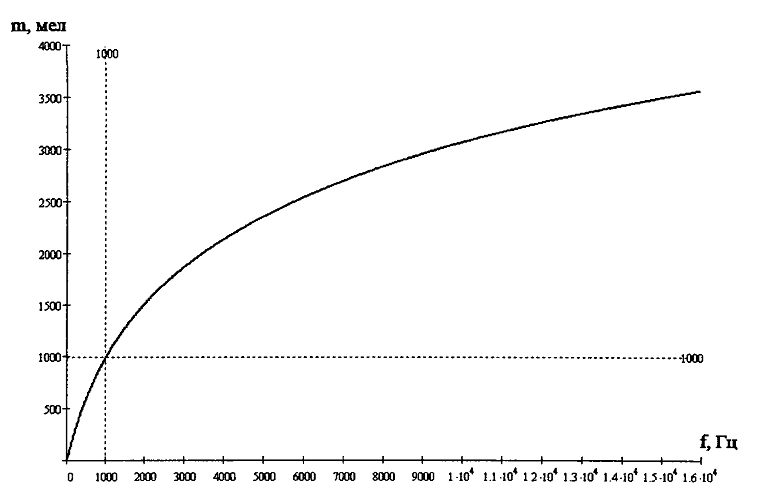
\includegraphics[scale=0.8]{pic-ear-04}
\caption{График соотношения между шкалами герц и мелов}
\label{pic-ear-04}
\end{figure}

Уже упомянутая нами единица измерения Барк, как и мел, является достаточно распространенной единицей измерения высоты тона. При этом шкалы барков и мелов очень близки. Одна из существующих эмпирических формул перевода герцев в барки выглядит следующим образом:

\[b [\text{Барк}]=13\arctan(0,00067f \text{[Гц]})+3,5\arctan((\frac{f \text{[Гц]}}{7500})^2),\]

где $f$~--- частота, измеренная в Гц, $b$~--- частота, измеренная в Барк.

Итак, частотные параметры звука могут измеряться в герцах, мелах и Барках. Герц~--- это единица измерения, которой удобно пользоваться при проведении спектрального анализа. Мел и Барк~--- это психофизиологические акустические единицы измерения высоты тона, используемые в психоакустике при оценке субъективной высотой тона. На рис. \ref{pic-ear-05} показан график соотношения трех шкал: шкала барков (сплошная линия), шкала мелов (пунктирная линия) и шкала герц (совпадает с осью абсцисс). Для удобства сравнения графиков шкалы барков и мелов нормализованы (т.е. масштабированы так, что максимальным значением на шкалах является единица).

\begin{figure}[ht]
\centering
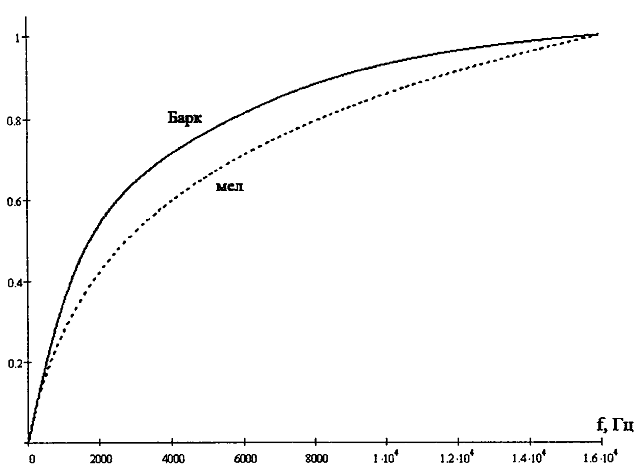
\includegraphics[scale=0.8]{pic-ear-05}
\caption{График соотношения трех шкал}
\label{pic-ear-05}
\end{figure}

Как видно из графика, шкалы барков и мелов приблизительно совпадают, хотя некоторые расхождения наблюдаются в области средних частот.

Длительность звука сказывается на высоте тона критическим образом. Так, очень кратковременное звучание (менее 15 мс) любой частоты покажется на слух просто резким щелчком - человек не сможет различить высоту тона для такого сигнала. Высота тона начинает восприниматься лишь после 15 мс для частот в полосе 1000-2000 Гц и лишь спустя 60 мс - для частот ниже 500 Гц. Это явление называется инерционностью слуха. Инерционность слуха связана с устройством базилярной мембраны. Кратковременные звуковые всплески не могут заставить
мембрану резонировать на нужной частоте, а значит, мозг не получает информацию о высоте тона при очень коротких звуках. Минимальное время, требуемое для распознавания высоты тона, зависит от частоты звукового сигнала, а точнее~--- от длины звуковой волны. Чем выше частота звука, тем меньше длина звуковой волны и тем меньше инерционность слуха, т.е. тем быстрее мозг улавливает звуковые колебания.

В природе мы почти не сталкиваемся с чистыми тонами. Звучание любого музыкального инструмента является сложным и состоит из множества частотных составляющих. Как мы сказали выше, даже при очень сложных звуковых колебаниях слух человека способен распознать высоту звучания. Тем не менее даже при одинаковой высоте тона звучание, например, скрипки отличается на слух от звучания рояля. Это связано с тем, что, помимо высоты звучания, слух способен оценивать также "<окрас"> звучания, т.е. его тембр. 

{\itshape Тембром звука} называется такое качество звука, которое, вне зависимости от частоты и амплитуды, позволяет отличить одно звучание от другого. Тембр звука зависит от общего спектрального состава звука и соотношения амплитуд составляющих спектра и фактически не зависит от высоты основного тона. Другими словами, тембр звука с одним и тем же основным тоном определяется составом обертонов (их частотами и амплитудами), а также характером нарастания амплитуд в начале звучания и их спадания в конце звучания. Немалое влияние на воспринимаемый тембр звучания оказывает явление инерционности слуховой системы. Оно выражается, например, в том, что на распознавание тембра слуховой системе требуется около 200 мс. На рис. 3.6 представлены сигналограммы двух звуковых сигналов~--- трубы и фортепиано.

\begin{figure}[h]
\centering
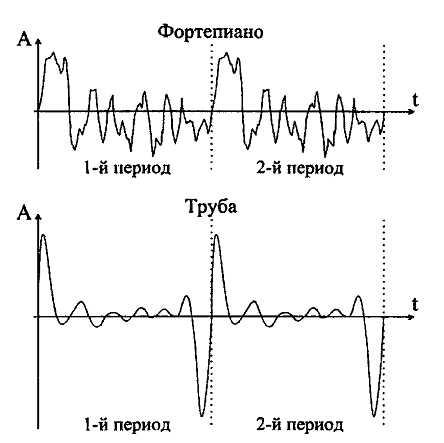
\includegraphics[scale=0.8]{pic-ear-06}
\caption{ Сигналограммы звучания трубы и фортепиано}
\label{pic-ear-06}
\end{figure}

Оба звуковых сигнала представляют собой запись ноты "<ля"> первой октавы. Высота тона у обоих сигналов одинакова и определяется периодом колебаний (оба графика вмещают ровно по два периода колебаний). Тем не менее слух совершенно ясно отличает звучание одного инструмента от другого благодаря разнице в форме периода (т.е. разнице в формах кривых в пределах периода).

Надо заметить, что сама по себе воспринимаемая высота тона тоже зависит от тембра звука. Так, например, высота тона для звуков с богатым спектром определяется слуховой системой даже в том случае, если из них удалить основной тон.

\subsection{Интенсивность и громкость звука}
Интенсивность звуковой волны (сила звука)~--- это параметр, характеризующий звук не как психофизиологическое, а как физическое явление. Однако между интенсивностью и громкостью звука существует тесная взаимосвязь, а именно~--- уровень громкости звука является функцией его интенсивности и частоты. 

{\itshape Интенсивностью звука} (или {\itshape силой звука}) называется количество звуковой энергии $W_\text{з}$ переносимой звуковой волной за единицу времени $t$ через единицу
площади поверхности $S$, нормальной к направлению распространения звуковой волны:

\[I=\frac{W_\text{з}}{St}=\frac{N_\text{з}}{t}\, \text{Вт}/\text{м}^2\]
где $N_\text{з}$~--- звуковая мощность, Вт; $W_\text{з}$~--- звуковая энергия, Дж; $S$~--- площадь поверхности, перпендикулярной к направлению распространения звуковой волны (звука), $m^2$.

Мерой силы слухового ощущения является громкость звука. {\itshape Громкость звука}~--- это психофизиологическая характеристика восприятия звука, определяющая ощущение интенсивности (силы звука), т.е. {\itshape громкость звука является мерой силы слухового ощущения}. 

Громкость звука нарастает непропорционально увеличению интенсивности сигнала. На ощущаемую громкость влияют величина звукового давления, частота и длительность звукового сигнала. Чтобы правильно судить о связи ощущения звука (его громкости) с раздражением (уровнем силы звука), нужно учитывать, что интенсивности звука соответствует ощущение громкости звука,
которое возрастает значительно медленнее, чем увеличивается сила звука, подчиняясь {\itshape закону Вебера-Фехнера}: {\itshape прирост силы ощущения пропорционален логарифму отношения интенсивностей двух сравниваемых раздражений}.

Величина, оценивающая громкость звука,~--- это уровень интенсивности звука $L_I$ который определяется соотношением

\[L_I=k \log_{10}{\frac{I}{I_0}}, \text{дБ}\]
где $I$~--- измеряемая интенсивность (сила) звука, $\text{Вт}/\text{м}^2$; $I_0\approx 10^{-12} \text{Вт}/\text{м}^2$~--- интенсивность самого слабого звука, воспринимаемого человеческим ухом, принятая за {\itshape порог интенсивности} (т.е. за нижний предел чувствительности (слышимости) человеческого уха); $k$~--- коэффициент пропорциональности: при $k=1$ уровень звука выражается в белах, при $k=10$ уровень звука выражается в децибелах.

На практике используется единица "<децибел"> , так как минимальный прирост громкости, воспринимаемый ухом, примерно равен 1 дБ.

Эффективное звуковое давление может быть рассчитано по следующей формуле:
\[P_{\text{эф}}=\sqrt{I \rho C}.\]

Величину \(P_{0~\text{эф}}=2\cdot10^{-5}\ \text{Н}/\text{м}^2\) называют порогом звукового давления; это наименьшая величина эффективного звукового давления, соответствующая порогу интенсивности $I_0$.

{\itshape Порогом слышимости} принято называть то наименьшее значение величины эффективного звукового давления, при котором звук еще воспринимается органами слуха. Порог слышимости также зависит от частоты звука и может достигать своего минимального значения в широком диапазоне частот ($700-6000$ Гц). Поэтому принят так называемый стандартный порог слышимости, соответствующий частоте $f=1000$ Гц.

\begin{figure}[h]
\centering
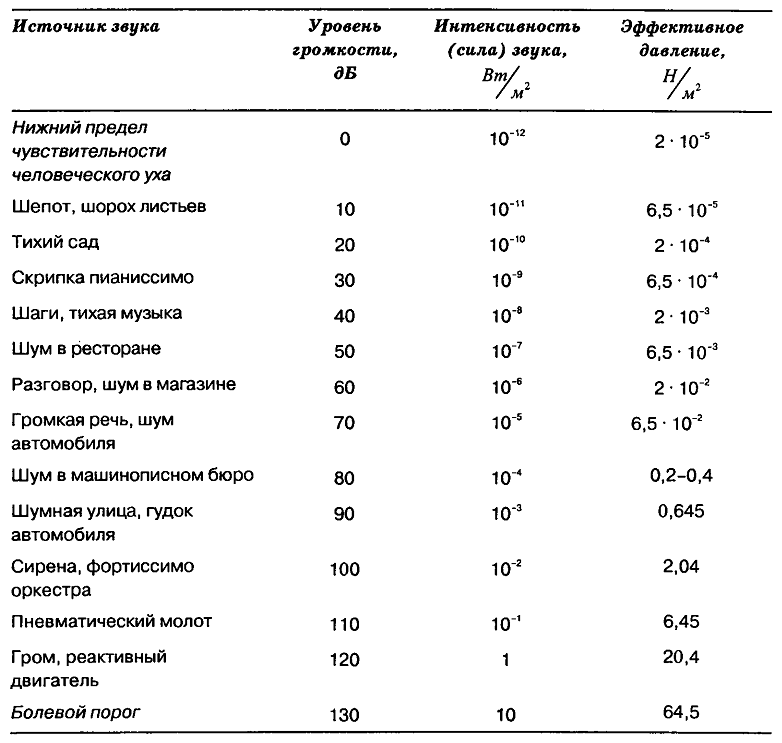
\includegraphics[scale=0.8]{pic-ear-07}
\caption{Приблизительные значения уровней громкости звуков}
\label{pic-ear-07}
\end{figure}

Используя закон Вебера-Фехнера и на основе экспериментальных исследований Флетчера и Мансона, которые изучали восприятие человеком громкости чистых тонов на различных частотах, была построена известная шкала единиц измерения громкости звука~--- так называемые кривые равной громкости (рис. \ref{pic-ear-08}).

\begin{figure}[h]
\centering
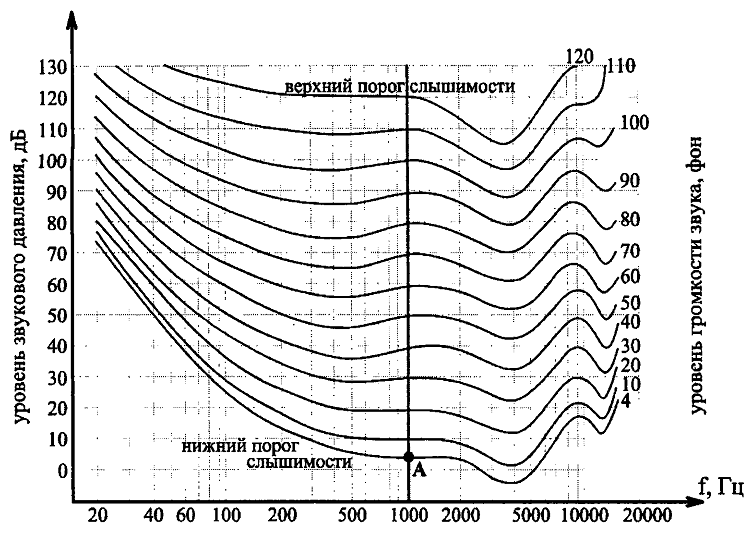
\includegraphics[scale=0.8]{pic-ear-08}
\caption{Кривые равной громкости}
\label{pic-ear-08}
\end{figure}

По этой шкале измеряется не абсолютное значение громкости, а уровень громкости звука, который отсчитывается от условного нуля (аналогично уровню звукового давления). За условный нуль громкости принимается громкость эталонного звука при частоте 1000 Гц и звуковом давлении $2\cdot10^{-5}~\text{Н}/\text{м}^2$. При этом единицей измерения уровня громкости является фон. 

Под одним {\itshape фоном} (от англ. "<рhon">) следует понимать уровень громкости звука, для которого уровень звукового давления равногромкого с ним звука частоты 1000 Гц равен 1 дБ. 
Чтобы выразить уровень громкости какого-либо звука, необходимо сравнить его с уровнем
громкости звука на эталонной частоте 1000 Гц. 

Кривые равной громкости, представленные на рис. \ref{pic-ear-08}, показывают, что человек (среднестатистический) начинает слышать звук с определенного значения уровня звукового давления, и на различных частотах уровень звукового давления, начиная с которого звук воспринимается ухом, оказывается различным.

Существует еще одна относительная единица измерения уровня громкости звука~--- сон (от лат. "<sonus">~--- "<звук">). Уровень громкости величиной 1 сон соответствует уровню громкости 40 фон при частоте звука 1000 Гц. При каждом увеличении громкости звука на 10 фон число единиц "<сон">  приблизительно удваивается. График отношения шкалы сонов и шкалы фонов представлен на рис. \ref{pic-ear-09}.

\begin{figure}[h]
\centering
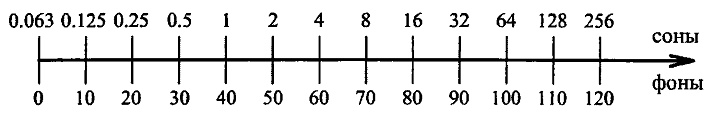
\includegraphics[scale=0.8]{pic-ear-09}
\caption{Шкала сонов и шкала фонов}
\label{pic-ear-09}
\end{figure}

Под конец рассматриваемой темы заметим, что под уровнем громкости на практике иногда подразумевают уровень интенсивности звука. Для достаточно мощных источников звука такая путаница понятий вполне справедлива~--- различие между субъективной громкостью и ее уровнем (интенсивностью) для таких источников невелико, в то же время для источников малой мощности это различие становится большим. Заметим также, что субъективная громкость природных сигналов выше, чем субъективная громкость чистых тонов той же интенсивности.

\subsection{Порог слышимости и маскировка}
Уровни равной громкости звука для слуха человека не остаются постоянными с изменением частоты, т.е. чувствительность слуховой системы человека зависит как от громкости звука, так и от его частоты. И порог слышимости также не одинаков на разных частотах, например порог слышимости сигнала на частоте около 3 кГц составляет приблизительно 0 дБ, а на частоте 200 Гц~--- около 15 дБ. Напротив, {\itshape болевой порог слышимости} мало зависит от частоты звука и колеблется в пределах 110-130 дБ.

Порогом болевого ощущения называется то наибольшее эффективное давление звука, при кото-ром восприятие звука еще не вызывает болевого ощущения. Если эффективное давление звука превосходит эту величину, то нормальное восприятие звука становится невозможным.

График порога слышимости представлен на рис. \ref{pic-ear-10}. Обратим внимание, что, поскольку острота слуха с возрастом меняется, график порога слышимости в верхней полосе частот различен для разных возрастов. Частотные составляющие с амплитудой ниже порога слышимости (т.е. находящиеся под графиком порога слышимости) оказываются незаметными на слух.

\begin{figure}[h]
\centering
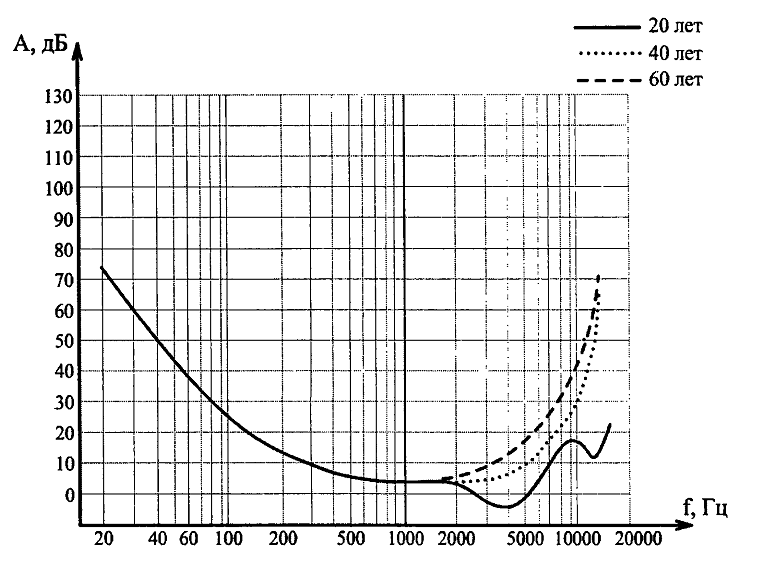
\includegraphics[scale=0.8]{pic-ear-10}
\caption{График порога слышимости для различных возрастов слушателя}
\label{pic-ear-10}
\end{figure}

На рис. \ref{pic-ear-11} представлена диаграмма слуховых восприятий, на которой приблизительно показаны области громкости речи и музыки, а также порог риска и болевой порог. Кривая порога слышимости, по сути, представляет собой кривую равной громкости для минимальной воспринимаемой громкости и соответствует приблизительно 4 фонам.

\begin{figure}[h]
\centering
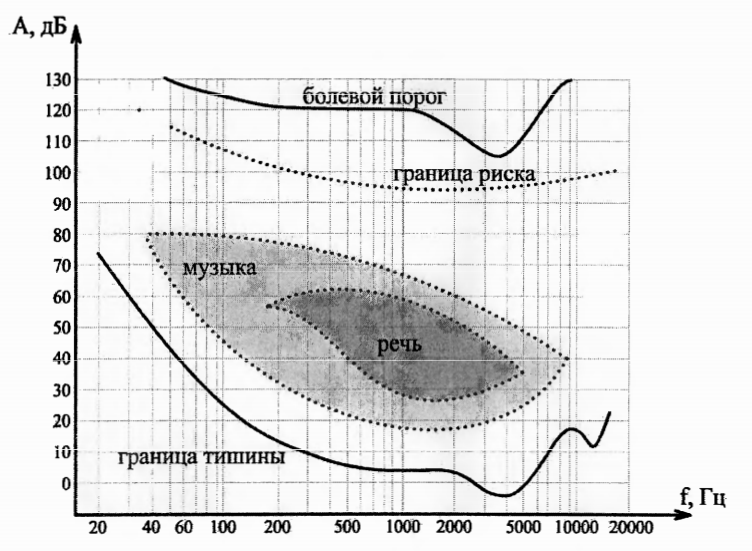
\includegraphics[scale=0.8]{pic-ear-11}
\caption{Диаграмма слуховых ощущений}
\label{pic-ear-11}
\end{figure}

Интересным и исключительно важным является тот факт, что порог слышимости слуховой системы, так же как и кривые равных громкостей, является непостоянным в разных условиях. Представленные выше графики порога слышимости справедливы для полной тишины. В случае проведения опытов по измерению порога слышимости не в полной тишине, а, например, в зашумленной комнате или при наличии какого-то постоянного фонового звука, графики окажутся другими. 

Это и не удивительно. Идя по улице и разговаривая с собеседником, мы часто вынуждены прерывать свою беседу, когда мимо нас проезжает какой-нибудь грузовик, поскольку шум грузовика не дает нам слышать собеседника. Этот эффект называется частотной маскировкой. 

На рис. \ref{pic-ear-12} схематично показано, каким образом чистый тон частоты $f_m$ создает маскирующий эффект и видоизменяет кривую порога слышимости в тишине.

\begin{figure}[h]
\centering
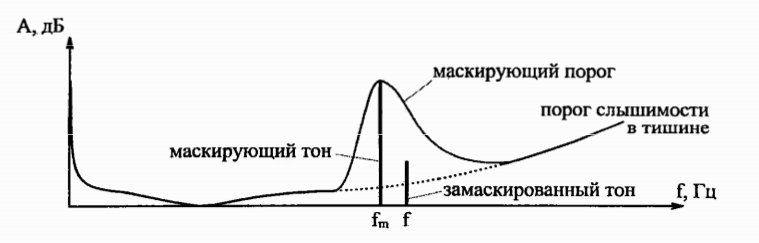
\includegraphics[scale=0.8]{pic-ear-12}
\caption{Эффект частотной маскировки}
\label{pic-ear-12}
\end{figure}

Как видно из рисунка, присутствие чистого тона при проведении измерений порога слышимости ощутимо видоизменяет его график (сплошная линия) по сравнению с тем же опытом, проведенным в тишине (пунктирная линия). Частотная составляющая $f$  имеет амплитуду выше порога слышимости в тишине, а значит, была бы отчетливо слышна в условиях тишины. Наличие же маскирующего тона $f_m$ изменяет порог слышимости, "<накрыв"> его маскирующим порогом (следует отметить несимметричность формы маскирующего порога: в сторону увеличения частоты он более пологий). 

В результате частота $f$ оказывается ниже порога слышимости и на слух не ощущается (в то время как сама составляющая слышна хорошо). Говорят, что частота $f_m$ маскирует частоту $f$. 

Конечно, приведенный пример является одним из простейших, однако он наглядно демонстрирует эффект частотной маскировки. График маскирующего порога может оказаться куда более сложным
при наличии нескольких маскирующих тонов разных амплитуд и частот.

Рассмотренный нами эффект частотной маскировки справедлив для частотных составляющих, присутствующих в спектре сигнала в одно и то же время. Однако ввиду инерционности слуха эффект маскировки может простираться и во времени.

В частности, одна частотная составляющая может маскировать другую частотную составляющую даже тогда, когда они появляются в спектре не одновременно, а с некоторой задержкой во времени. Этот эффект называется частотно-временной маскировкой. В случае, когда маскирующий тон прекращается во времени раньше появления маскируемого тона, эффект называют постмаскировкой. В случае же, когда маскирующий тон появляется позже маскируемого (возможна и такая маскировка), эффект называется пред маскировкой.

Временная предмаскировка является вполне логичным эффектом, поскольку, как мы говорили, слушателю нужно некоторое время, чтобы начать ощущать тот или иной тон (объяснение этому снова кроется в механизме принципа действия базилярной мембраны, которая не всегда успевает среагировать на очень кратковременное возбуждение). В случае же, когда еще до нужного момента тон оказывается замаскированным другим тоном, слух так и не успевает зафиксировать присутст-
вие замаскированного тона, и последний оказывается неуслышанным.

Постмаскировка также объясняется инерционностью слуха. Для переключения слуха с восприятия одного тона на восприятие другого требуется некоторое время.

Некоторый (маскирующий) тон даже после его исчезновения как бы "<продолжает звучать">
 в голове слушателя еще определенный промежуток времени (время затухания колебаний базилярной мембраны). Если за этот промежуток времени успевает появиться и исчезнуть некоторый близкий к предыдущему по частоте тон, то он оказывается замаскированным, т.е. незамеченным органами слуха.

На рис. \ref{pic-ear-13} продемонстрирован эффект маскировки во времени в виде диаграммы, иллюстрирующей длительность и уровень маскировки в случае пред- и постмаскировки.

\begin{figure}[h]
\centering
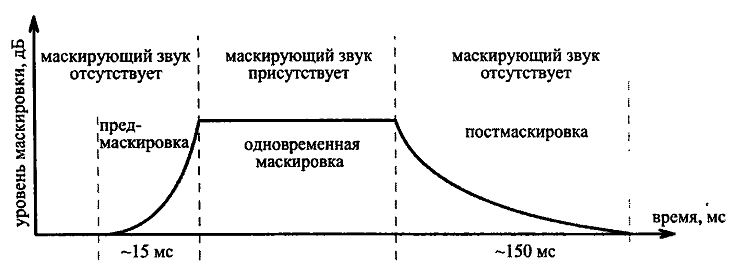
\includegraphics[scale=0.8]{pic-ear-13}
\caption{Диаграмма временной маскировки}
\label{pic-ear-13}
\end{figure}

Из диаграммы видно, что эффект предмаскировки появляется приблизительно за 15 мс до маскирующего тона. Начиная с момента появления маскирующего тона имеет место одновременная (частотная) маскировка. После исчезновения маскирующего тона на протяжении еще приблизительно 150 мс можно наблюдать эффект постмаскировки. Естественно, значения времени усреднены и могут сильно меняться в зависимости от частоты маскирующего тона.

Эффект частотной маскировки, а также понятия порога слышимости и маскирующего порога являются ключевыми и широко используются в самых различных технологиях сжатия цифровых аудиоматериалов.

\section{Восприятие пространственности звука}
Человек способен определять, откуда слышен звук. Эту способность называют {\itshape бинауральным эффектом}. Бинауральный эффект можно объяснить, исходя из основных положений физиологической акустики. Уши человека расположены на определенном расстоянии "<по ширине головы">. Сигнал, приходящий от источника звука, находящегося напротив слушателя, приходит в оба уха одновременно, и слуховой аппарат (мозг) интерпретирует это, как расположение источника сигнала либо позади, либо спереди, но не сбоку. Если же сигнал приходит от источника, смещенного относительно центра головы, то звук попадает в одно ухо быстрее, чем
во второе, что позволяет мозгу соответствующим образом фиксировать это, как прием сигнала слева или справа, и даже приблизительно определять угол направления, в котором находится источник звука. Слуховой аппарат человека способен определить направление звукового сигнала по разнице во времени попадания сигнала в левое и правое ухо в пределах до 1 мс. Такой способ определения направления используется слуховым аппаратом (мозгом) в полосе частот $300-1000$~Гц.

Направление, в котором находится источник звука в полосе частот выше 1000~Гц, определяется мозгом человека путем анализа громкости звука. Дело в том, что звуковые волны с частотой выше 1000~Гц сравнительно быстро затухают в пространстве. Поэтому амплитуды звуковых волн, доходящих до левого и правого ушей слушателя, довольно заметно отличаются, что позволяет мозгу определять направление прихода сигнала по разнице громкостей. Немаловажной здесь является способность человека поворачивать голову в сторону кажущегося источника звука. Эта способность является естественным механизмом контроля правильности определения направления, в котором находится источник звука.

На рис. \ref{pic-ear-14} показан источник звука, смещенный влево относительно центра
головы слушателя. Поскольку расстояние $L_L$ от левого уха до источника меньше, чем соответствующее расстояние $L_R$ до правого уха, то звук от источника приходит быстрее в левое ухо, и, кроме того, в нем же звук кажется громче. Несмотря на кажущуюся незначительную разницу в расстояниях $L_L$ и $L_R$, слуховая система человека все же фиксирует эту разницу и слушатель, даже закрыв глаза, может вполне уверенно определить, что звук приходит к нему слева.

\begin{figure}[h]
\centering
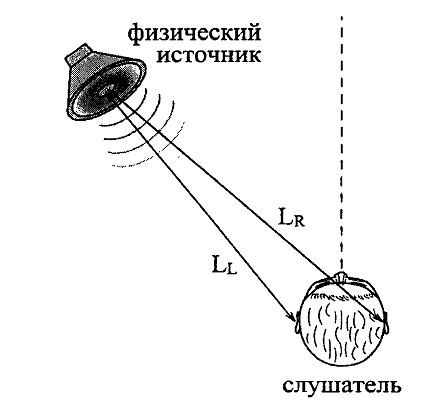
\includegraphics[scale=0.8]{pic-ear-14}
\caption{Физический источник расположен слева от слушателя}
\label{pic-ear-14}
\end{figure}

Способность слухового аппарата человека определять направление звукового сигнала по разнице во времени прихода сигнала в левое и правое ухо, а также способность идентифицировать разницу в интенсивности слухового ощущения, вызываемого звуковой волной в левом и правом ушах, используется в стереофонии.

{\itshape "<Стереофония">} происходит от греч. "<stereos">~--- "<объемный">, "<пространственный">. "<Стереофония"> в устаревшей, но наиболее верной трактовке~--- донесение до слушателя пространственного звучания; в более современной (но исторически искаженной трактовке)~--- донесение до слушателя звуковой картины с помощью двухканальной системы.

Так, имея два физических источника звука, можно создать у слушателя ощущение наличия мнимого источника звука, расположенного между двумя физическими.

Причем этот мнимый источник звука можно "<расположить"> в любой точке на линии, соединяющей два физических источника. Для этого нужно воспроизвести одну аудиозапись (например, фонограмму со звуком рояля) через оба физических источника, но сделать это с некоторой временной задержкой в одном из них и соответствующей разницей в громкости. Изменяя указанную временную задержку (увеличивая или уменьшая) в одном из физических источников и одновременно изменяя в этом источнике громкость звука (соответственно увеличивая или уменьшая), можно менять расположение мнимого источника звука на упомянутой выше мнимой линии. Мнимая линия, соединяющая два физических источника звука при воспроизведении звукового сигнала, на которой располагаются мнимые источники звука, называется {\itshape стереобазой}.

Предположим, что два динамика расположены перед лицом слушателя и расставлены по сторонам под равными углами к слушателю (рис. \ref{pic-ear-15}).

\begin{figure}[h]
\centering
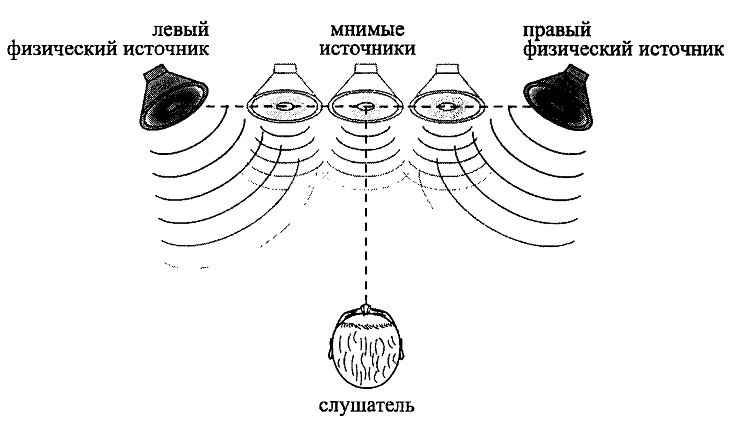
\includegraphics[scale=0.8]{pic-ear-15}
\caption{Диаграмма восприятия слушателем звуковой стереокартины}
\label{pic-ear-15}
\end{figure}

Теперь воспроизведем одновременно (т.е. с нулевой временной задержкой) и с одинаковой громкостью одну и ту же запись через оба источника. Поскольку время прихода сигнала в оба уха слушателя (так же, как и громкость сигналов справа и слева) одинаково, у слушателя создастся ощущение, что источником звука является точка пространства, расположенная ровно по центру между динамиками. 

Проведем этот же эксперимент, задержав сигнал в левом динамике на 0,5 мс и немного ослабив его амплитуду. В результате мнимый источник звука сдвинется с точки зрения слушателя вправо, так как сигнал придет в правое ухо слушателя раньше, чем в левое, и будет слышен в нем громче. Дальнейшее увеличение временной задержки и соответствующее понижение громкости сильнее сдвигает мнимый источник вправо (рис. \ref{pic-ear-16}).

\begin{figure}[h]
\centering
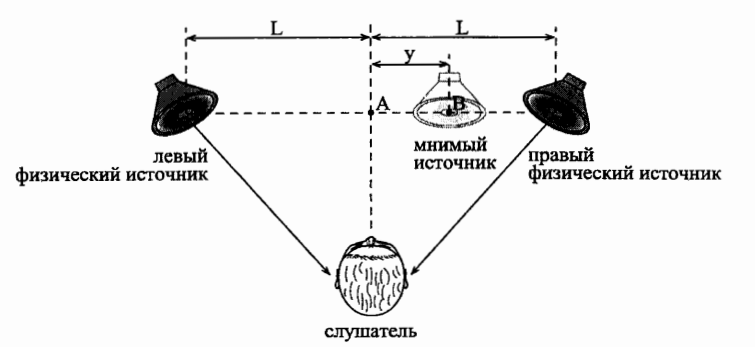
\includegraphics[scale=0.8]{pic-ear-16}
\caption{Диаграмма восприятия слушателем звуковой стереокартины. Мнимый источник сдвигается вправо}
\label{pic-ear-16}
\end{figure}

Используя описанный бинауральный эффект, можно при помощи двухканальной аудиозаписи и соответствующего воспроизведения донести до слушателя почти такую же картину звучания, какую он ощутил бы сам, если бы лично присутствовал, например, на каком-нибудь концерте. 

Действительно, представим себе, что мы установили два микрофона (каждый из которых осуществляет независимую запись) на равных расстояниях от центра оркестровой ямы (рис. \ref{pic-ear-17}).

\begin{figure}[h]
\centering
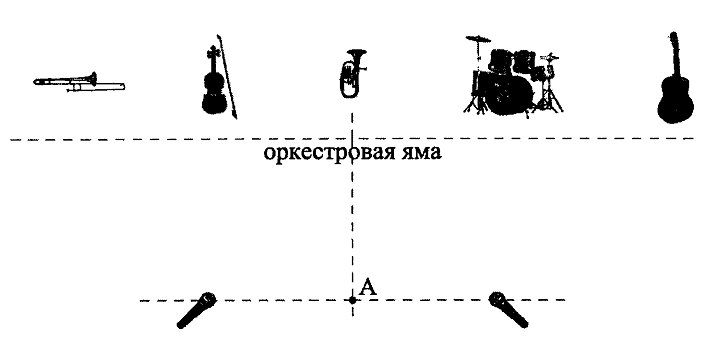
\includegraphics[scale=0.8]{pic-ear-17}
\caption{Запись звучания оркестра с помощью двух микрофонов}
\label{pic-ear-17}
\end{figure}

Тогда, как следует из рисунка, звук альта будет приходить в оба микрофона одновременно и слышаться в них одинаково громко; звук скрипки будет приходить в левый канал записи чуть раньше, чем в правый, и звучать слева чуть громче; звук гитары будет хорошо слышен в точке, где расположен правый микрофон, и почти не слышен в точке, где расположен левый, и т.д. 

Теперь, если полученные от обоих микрофонов аудиозаписи воспроизвести с помощью двух правильно расставленных перед слушателем динамиков (см. рис. \ref{pic-ear-16}), звук гитары будет идти только из правого динамика, звук альта~--- из обоих одновременно, а звук скрипки~--- из левого раньше и громче, чем из правого. 

Таким образом, мнимый оркестр как бы расположится на невидимой линии, соединяющей два динамика, а вместо микрофонов перед центром оркестровой ямы (точка А на рис. \ref{pic-ear-17}) будет стоять сам слушатель. При этом слушатель получит почти полное представление о "<живом"> звучании оркестра. Такая (мысленно проделанная нами) двухканальная запись называется стереофонической, а ширина, которую занимает мнимый оркестр на пространственной стереокартине, называется шириной стереопанорамы.

{\itshape Стереопанорама}~--- это воображаемая слушателем поверхность излучения звуковых волн. Стереопанорама является частью стереобазы. Ширина стереопанорамы является максимально возможной при данном конкретном расположении физических источников звука, если она равняется
ширине стереобазы (исключая специальные искусственные методы мнимого расширения стереопанорамы).

Если осуществить запись звукового сигнала с помощью одного приемника (микрофона), то при воспроизведении этого сигнала через один или даже несколько динамиков слушатель не сможет ощутить пространственность оригинального звучания, поскольку записанный сигнал есть монофоническая запись (одноканальная запись), т.е. запись оригинального звучания, сделанная лишь из одной точки пространства.

Качество донесения до слушателя оригинальной пространственной звуковой картины можно повышать путем добавления в запись дополнительных каналов (трех- и более канальная запись), осуществляя одновременно несколько отдельных записей в трех (и более) разных точках пространства.

\section{Музыкальный звук и шумы}
\subsection{Музыкальный звук}
Понятие "<слышимый звук"> можно трактовать и понимать широко: это и музыкальный звук, и шумы, и человеческая речь, и звуки живой природы, животных, зверей, птиц и т.д. и т.п. По каждой из перечисленных тем можно проводить отдельные обширные исследования, писать статьи, книги и т.д. В этом разделе мы кратко остановимся на рассмотрении музыкального звука. Рассмотрим отличительные особенности музыкального звука от перечисленных выше звуков. 

{\itshape Музыкальный звук}~--- это звук тональный, имеющий так называемый линейчатый дискретный частотный спектр (в отличие от шумов, имеющих так называемый сплошной частотный спектр). Это значит, что взятый конкретный фрагмент музыкального звука состоит из набора звуков, дискретных по частоте, т.е. частоты заполняют этот фрагмент с определенным интервалом или между собой, или между определенными группами частот. 

Почему в основу построения музыкального звука заложена дискретность по частоте набора звуков?  Это связано с природными особенностями и возможностями слухового аппарата человека к восприятию звука вообще и музыкального звука в частности. Если несколько детализировать сказанное, то можно
выделить следующие основные причины, относящиеся к психофизиологическим
особенностям восприятия музыкального звука человеком: 
\begin{itemize}
\item инерционность слухового аппарата человека;
\item избирательность в распознавании низких и высоких частот в звуковом частотном спектре;
\item способность памяти человека лучше распознавать, усваивать и запоминать дискретную по частоте аудиоинформацию.
\end{itemize}

Существует еще одна причина, которая обусловлена возможностями музыкальных инструментов, а именно~--- большинство музыкальных инструментов не позволяет извлекать с их помощью звуки произвольной высоты и ограничивают музыканта 
конкретным набором дискретных значении высоты тона.

{\itshape Тон в музыке}~--- это звук, обладающий определенной высотой звучания. В современной 12-тоновой музыкальной системе различают целый тон~--- расстояние между двумя звуками, равное 1/6 октавы, и полутон~--- наименьшее расстояние между двумя звуками.

{\itshape Октава} (от лат. "<octava">~--- "<восьмая">)~--- один из музыкальных интервалов или часть музыкального звукоряда, в которую входят все звуки музыкальной системы. Высоты крайних звуков октавы различаются на слух ровно вдвое.

Музыкальный звук характеризуется определенной {\itshape высотой} (от 16~Гц до 4,5~кГц), {\itshape громкостью}, {\itshape длительностью} и {\itshape тембром}. 

{\itshape Высота музыкального звука} относится к психофизиологическим параметрам, определяется каждым человеком субъективно и зависит, в основном, от частоты. С ростом частоты высота музыкального звука увеличивается.

{\itshape Громкость звука} вообще и музыкального звука в частности~--- это параметр, который также связан с психофизиологией восприятия звука человеком и является мерой силы слухового ощущения интенсивности (силы звука). Применительно к музыке под громкостью звука еще понимают различную относительную степень силы звучания голоса, инструмента, оркестра и т.д. В нотах громкость обозначают итальянскими терминами: {\itshape пиано} (от лат. "<piano">, сокращенно~--- Р)~--- тихо; {\itshape форте} (от лат. "<forte">~--- F)~--- громко и др.

{\itshape Длительность звукового сигнала}~--- это временн{\'a}я характеристика звучания.
В музыке существует такое понятие, как ритмическое деление длительности музыкального звука на равные части, которое лежит в основе ритмической организации музыки. Основной вид деления~--- это деление на две части: целой ноты на две половинные, половинной ноты на две четверти, четвертной - на две восьмые и т.д., а также деление трехдольных длительностей на три части.

Тембр музыкального звука характеризует его качество (окраску), определяемое положением формант в частотном спектре. Тембр музыкального звука зависит от того, какие обертоны сопутствуют основному тону, какова интенсивность каждого из них и в каких областях звуковых частот образуются их скопления (форманты). Чем качественнее музыкальный звук, тем более насыщена его окраска, тем лучше и точнее различаются звуки одинаковой высоты различных музыкальных инструментов.

Музыкальный звук лежит в основе построения так называемой {\itshape музыкальной
системы}, которая представляет собой высотную (интервальную) организацию музыкальных звуков на основе какого-либо единого принципа. Известны музыкальные системы из трех (трихорд~--- звукоряд из трех звуков), четырех (тетрахорд~--- 4-ступенный звукоряд), пяти (пентахорд), шести (гексахорд) и семи (диатоника) звуков в одной октаве. 

В настоящее время в музыке широкое распространение получила так называемая равномерно темперированная 12-ступенная музыкальная система (12-ступенный звукоряд). В этом звукоряде последовательно расположены семь полных и две неполные октавы. В каждую полную октаву входят 12 звуков, последовательно расположенных по высоте звучания (по высоте тона).

Название этой музыкальной системы ("<равномерно темперированная">) происходит от одного важного ее свойства: все тоны на музыкальной шкале находятся в строгой математической зависимости (от лат. "<temprere">~--- "<упорядочивать">).

Основой равномерно темперированной шкалы является нота "<ля"> первой октавы, имеющая частоту 440 Гц. Шкала содержит всего двенадцать полутонов и семь целых тонов (в одной октаве), обозначаемых "<до">, "<ре">, "<ми">, "<фа">, "<соль">, "<ля">, "<си"> (рис. \ref{pic-ear-18}).

\begin{figure}[h]
\centering
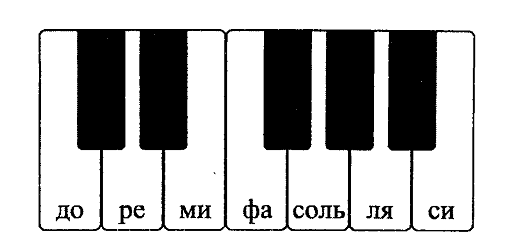
\includegraphics[scale=0.8]{pic-ear-18}
\caption{Ноты одной октавы на клавиатуре фортепиано}
\label{pic-ear-18}
\end{figure}

Шкала имеет единый интервальный коэффициент для всех интервалов, равный $\sqrt[12]{2} = 1,0595$. Это значит, что для вычисления частоты ноты $у$, зная частоту ноты $х$,
нужно умножить частоту ноты $х$ на число $(\sqrt[12]{2})^a$, где $а$~--- количество полутонов, отделяющих ноту $у$ от ноты $х$. Например, частота ноты "<си">  равна частоте "<ля"> (440~Гц~--- частота ее основной гармоники), умноженной на $(\sqrt[12]{2})^2$, т.е. 493,9~Гц.

Изменение частоты звуковых колебаний в определенном соотношении всегда приводит к изменению высоты тона на один и тот же музыкальный интервал. Рассмотрим пример: 
\begin{itemize}
\item Для ноты $C$ первой октавы частота равна 261,6Гц. 
\item Нота $E$ выше нее~--- 329,6Гц; разница в 68Гц.
\item Нота $C$ двумя октавами ниже~--- 65,4~Гц, а $E$ выше нее~--- 82,4~Гц; только на 17~Гц выше. 
\item Нота $C$ двумя октавами выше~--- 1046,5~Гц, а $E$ выше нее~--- 1318,5~Гц; т. е. выше на 272~Гц.
\end{itemize}

Несмотря на это переход от $C$ к $E$ звучит одинаково в каждом случае. Данный интервал~--- большая терция~--- звучат одинаково в разных позициях, хотя абсолютная разница между частотами изменяется, а вот отношение частот одинаково~--- около $1:1,25$.

Равенство интервального коэффициента для любых интервалов шкалы является важнейшим свойством равномерно темперированной шкалы. Оно позволяет, например, с легкостью транспонировать любую мелодию в любую тональность.

{\itshape Транспонирование}~--- перенесение музыкального произведения из одной тональности в другую.

Интересно заметить: октава равномерно темперированной шкалы имеет больше полутонов (двенадцать), чем любая другая принятая шкала, что позволяет музыкантам писать музыку, используя 84 тональности (в семи октавах). При этом частотная разрешающая способность слуховой системы человека, как мы говорили раньше, намного выше, и позволяет ему различать около 620 тональностей. Следовательно, равномерно темперированная шкала в этом смысле является далеко не идеальной, и, возможно, будут придуманы другие не менее удобные шкалы, обеспечивающие большую свободу действий.

\subsection{Шум и его разновидности}
Шум сопровождает человека везде. С этим явлением человек сталкивается в быту (это нежелательные звуки, мешающие отдыху, восприятию речи, музыки и т.д.), на работе (длительные монотонные или повторяющиеся кратковременные звуки, издаваемые рабочими механизмами), на улице (гул, скрежет, различного рода звуковые сигналы и пр.), на концерте, в театре (звуки, издаваемые при настройке музыкальных инструментов оркестра, многоголосный слабый гул в зале перед начетом спектакля, аплодисменты) и т.д. Можно приводить еще много других примеров, демонстрирующих явление шума. Так какое дать определение этому явлению? 

Медики, например, дали такое определение: шум~--- это звук, который оказывает вредное влияние на среднестатистического человека. И медики правы. Но с этим определением мы заходим в тупик, так как оно учитывает только физиологию человека. Есть другой подход к определению шума, и этот подход опирается на физическую основу звука, т.е. на состав амплитудно-частотного спектра. Ранее мы отмечали, что характер восприятия звука органами слуха человека зависит от состава спектра частот и в зависимости от этого звук может приобретать различную окраску и восприниматься, как тон или как шум. 

Если тональному звуку (речь, музыка, голос и т.д.) соответствует линейчатый (дискретный) спектр частот, то шумы обладают сплошным спектром, т.е. частоты такого спектра образуют непрерывный ряд значений и целиком (без каких-либо интервалов) заполняют некоторый звуковой фрагмент. И еще одна отличительная особенность шума~--- это в большинстве своем беспорядочные непериодические звуковые колебания, характеризующиеся случайными изменениями амплитуды, частоты и фазы звуковых волн, входящих в результирующую звуковую волну. 

В табл. \ref{table-noise-01} представлены примеры шумов с их приблизительными уровнями громкости.

\begin{table}[h]
  \caption{Примеры шумов с их приблизительными уровнями громкости}
  \begin{center}
  \begin{tabular}{|l|c|}
  \hline Пример шума & Уровень громкости, дБ \\
  \hline Тихая улица без транспорта & 30-35 \\
  \hline Городская улица с транспортом & 70-80 \\  
  \hline Авторемонтная мастерская & 80-90 \\  
  \hline Кузнечный цех & 100-110 \\    
  \hline Самолет на близком расстоянии & 120-130 \\   
  \hline   
  \end{tabular}
  \end{center}  
  \label{table-noise-01}
\end{table}

Несмотря на достаточную четкость сформулированных отличий шума от тонального звука, мы не можем провести на практике резкую границу между шумами и тонами, так как многие шумы все же обладают некоторым преимущественным тоном.

Рассмотрим некоторые из упоминаемых в профессиональной литературе разновидностей шумов.

\begin{itemize}
\item {\itshape Белый шум} (шум Джонсона). Такой шум имеет спектр с приблизительно постоянной спектральной плотностью на всей протяженности спектра. Сонограмма белого шума выглядит так, как показано на рис. \ref{pic-noise-01}.

\item {\itshape Розовый шум}. Спектр такого шума имеет спектральную плотность, уменьшающуюся на 3 дБ с каждой последующей октавой (спектральная плотность обратно пропорциональна частоте). На рис. \ref{pic-noise-02} представлена типичная сонограмма такого шума.

\item {\itshape Оранжевый шум}. Это квазипостоянный шум с конечной спектральной плотностью. Спектр такого шума имеет полоски нулевой энергии, рассеянные на
всей его протяженности. Такие полоски находятся около частот, соответствующих музыкальным нотам.

\item {\itshape Зеленый шум}. Подобен розовому шуму с усиленной областью частот в районе 500 Гц.

\item {\itshape Синий шум}. Его спектральная плотность увеличивается на 3 дБ с каждой последующей октавой (спектральная плотность пропорциональна частоте).

\item {\itshape Фиолетовый шум}. Это дифференцированный белый шум. Его спектральная
плотность увеличивается на 6 дБ с каждой последующей октавой (спектральная плотность пропорциональна квадрату частоты).

\item {\itshape Серый шум}. Спектр такого шума имеет график, аналогичный графику психоакустической кривой порога слышимости. Это значит, что для слухового
аппарата человека этот шум имеет одинаковую громкость на всем слышимом диапазоне частот.

\item {\itshape Коричневый шум}. Его спектральная плотность уменьшается на 6 дБ с каждой последующей октавой (спектральная плотность обратно пропорциональна квадрату частоты). На рис. \ref{pic-noise-03} представлена типичная спектрограмма коричневого шума.

\item {\itshape Черный шум}. Определений этого шума существует достаточно много. Мы остановимся на следующем. Черным шум~--- это сверхзвуковой белый шум. Такой шум имеет постоянную конечную спектральную плотность за пределами порога слышимости (20 кГц).
\end{itemize}

\begin{figure}[h]
\centering
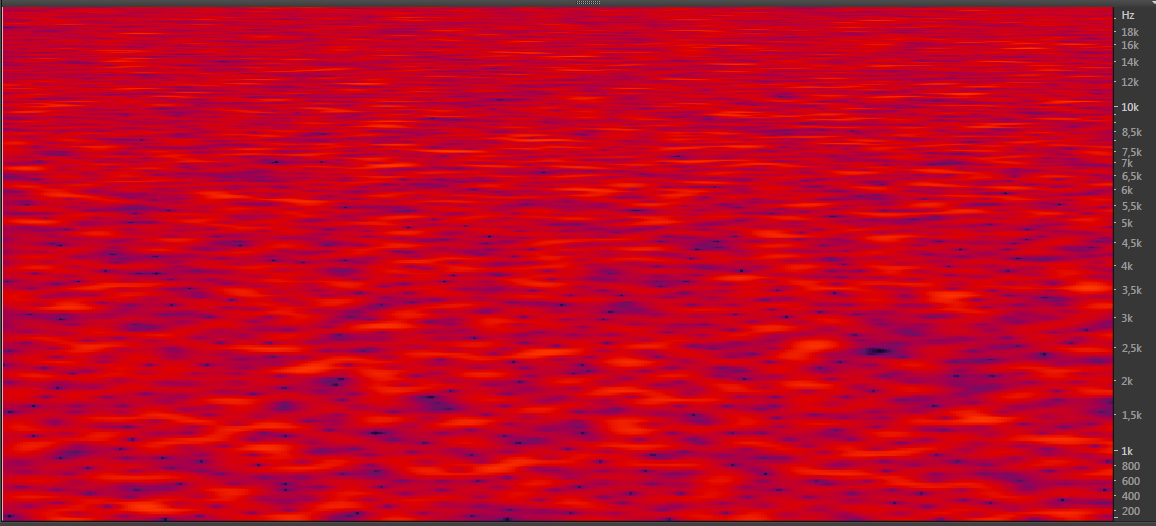
\includegraphics[scale=0.5]{pic-noise-01}
\caption{Типичная спектрограмма белого шума}
\label{pic-noise-01}
\end{figure}

\begin{figure}[h]
\centering
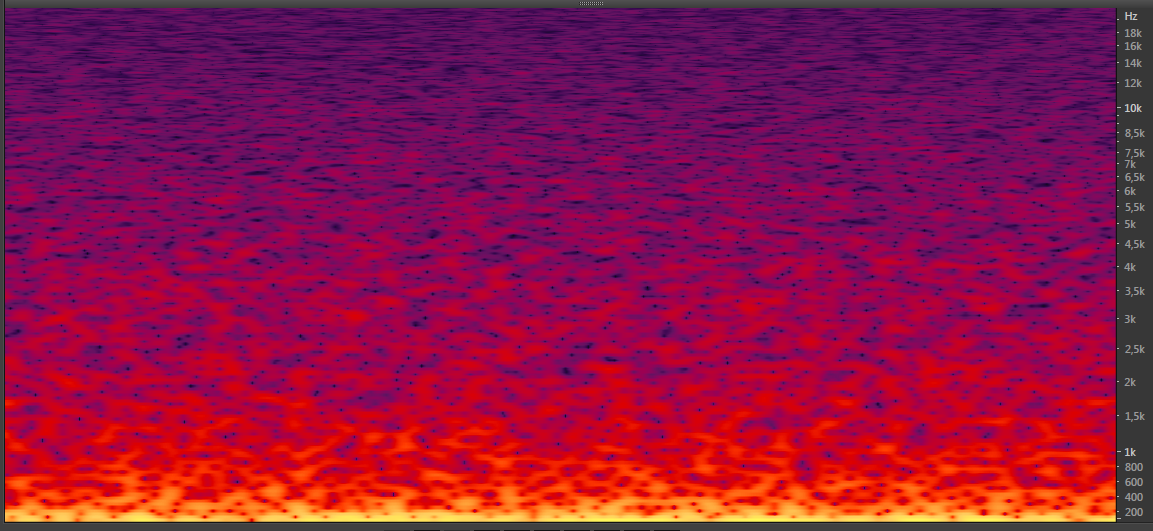
\includegraphics[scale=0.5]{pic-noise-03}
\caption{Типичная спектрограмма коричневого шума}
\label{pic-noise-03}
\end{figure}

\begin{figure}[h]
\centering
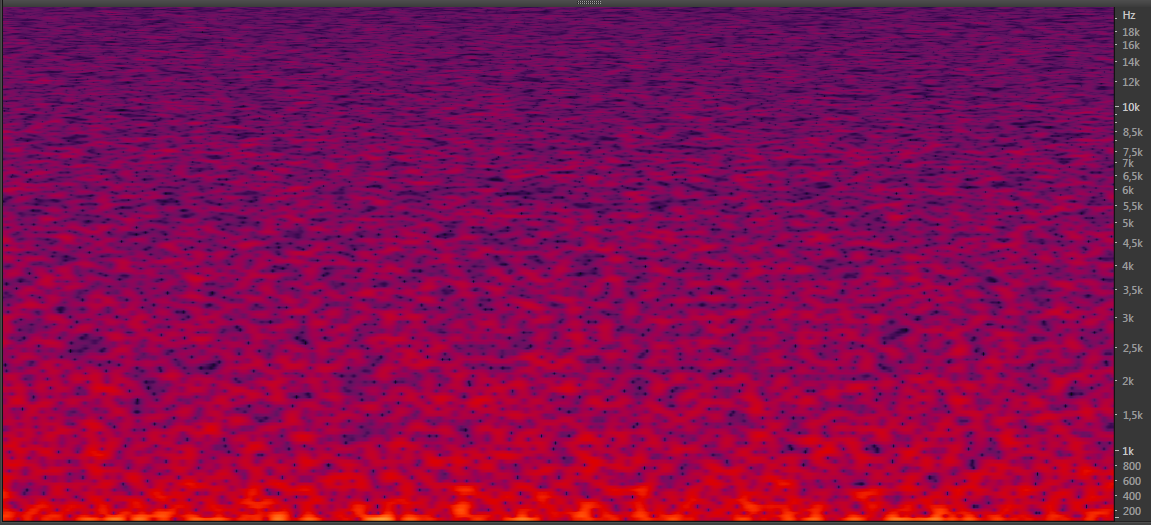
\includegraphics[scale=0.5]{pic-noise-02}
\caption{Типичная спектрограмма розового шума}
\label{pic-noise-02}
\end{figure}

Помимо рассмотренных "<цветных"> видов шумов, существует также понятие тонального шума. {\itshape Тональный шум}~--- это шум, в спектре которого имеются слышимые дискретные тоны. Шум считается тональным, если на частотах свыше 300 Гц уровень звукового давления в одной полосе шириной в треть октавы превышает уровни звукового давления в соседних полосах частот не менее чем на 10 дБ.

При описании характеристик различных звуковых сигналов, приборов и устройств часто употребляется понятие уровня шума. {\itshape Уровень шума}~--- это обобщенное понятие, которое может употребляться в отношении шумов и подразумевать как звуковое давление, так звуковую мощность и интенсивность (энергию) шумового звука.

Почти любая более или менее серьезная процедура, проводимая над звуковым сигналом, неизбежно ведет к его зашумлению. Шумы появляются и при записи, и при воспроизведении, и при обработке звука. При этом стоит отметить, что шум может оказаться как вредным, так и полезным.

В качестве простого наглядного примера влияния шумов на качество записи
аудиосигналов на рис.  \ref{pic-noise-04} представлена сигналограмма записи человеческой речи в малозашумленном помещении, а на рис.  \ref{pic-noise-05} для сравнения~--- эта же запись, но выполненная при наличии постоянной фоновой шумовой помехи (белый шум).

\begin{figure}[h]
\centering
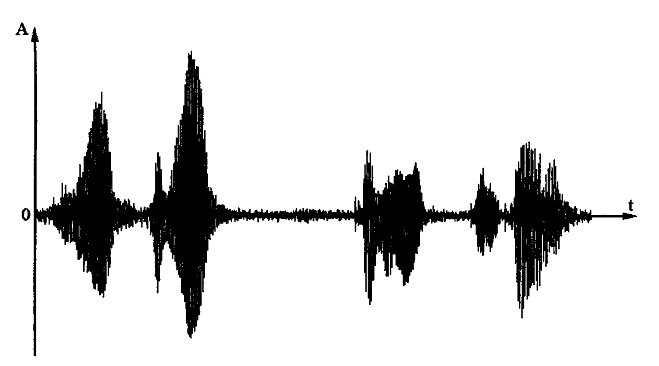
\includegraphics[scale=0.8]{pic-noise-04}
\caption{Сигналограмма записи речи в малозашумленном помещении}
\label{pic-noise-04}
\end{figure}

\begin{figure}[h]
\centering
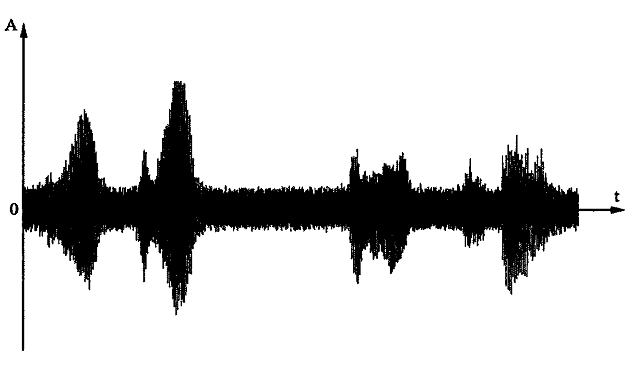
\includegraphics[scale=0.8]{pic-noise-05}
\caption{Сигналограмма записи речи в зашумленном помещении}
\label{pic-noise-05}
\end{figure}

Малая разница между уровнем полезного сигнала и уровнем фонового шума отрицательно сказывается на разборчивости и "<чистоте"> аудиоинформации при прослушивании. Нужно отметить, впрочем, что одной из психоакустических особенностей слуховой системы человека является ассоциативность слухового восприятия, которая помогает мозгу как бы "<отфильтровывать"> фоновые шумы на подсознательном уровне.

В отношении уровней шума и полезного сигнала часто пользуются понятием отношение сигнал/шум, сокращенно~--- С/Ш (Signal-to-Noise Ratio~--- SNR). Величина С/Ш показывает отношение уровня полезного сигнала к уровню шума.

Понятие С/Ш тесно связано с понятием динамического диапазона. В то время как динамический диапазон показывает соотношение максимального и минимального по уровню сигналов, С/Ш показывает отношение уровня шума к некоторому произвольному сигналу. По этой причине измерение С/Ш требует выбора опорного (эталонного) сигнала. В аудиоаппаратуре в качестве опорного сигнала часто выбирают синусоидальный сигнал. Аналогично динамическому диапазону отношение С/Ш обычно измеряется в децибелах. Естественно, чем выше значение С/Ш, тем лучше.

На рис. \ref{pic-noise-06} приведена иллюстрация отношения С/Ш на выходе некоторого аудиоустройства (например, усилителя мощности).

\begin{figure}[h]
\centering
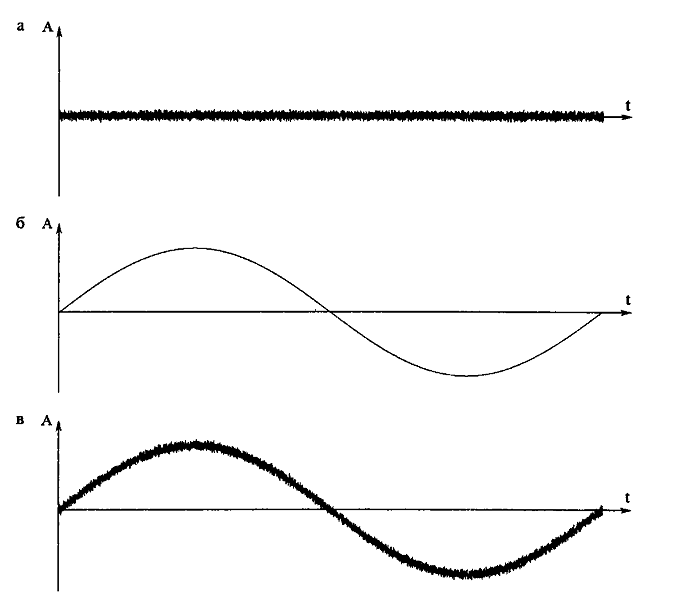
\includegraphics[scale=0.7]{pic-noise-06}
\caption{Иллюстрация С/Ш}
\label{pic-noise-06}
\end{figure}

На графике "<а"> показана сигналограмма сигнала на выходе устройства в отсутствие полезного сигнала. Сигналограмма представляет собой шум некоторого уровня $N$. 

На вход устройства подается чистая синусоида (график "<б">), после чего на выходе
устройства регистрируется сигнал уровня $S$, форма которого представлена на графике "<в">. Как видно из графика, это "зашумленная" синусоида, получившаяся в результате наложения внутреннего шума устройства на входной сигнал. Отношение
С/Ш устройства рассчитывается по формуле

\[SNR=20 \log_{10}{\frac{S}{N}}, \text{дБ.}\]

В качестве примера в табл. 3.4 представлены приблизительные значения соотношения С/Ш для некоторых типов аудиоаппаратуры.

\begin{table}[ht]
  \caption{Отношение С/Ш для некоторых типов аудиоаппаратуры}
  \begin{center}
  \begin{tabular}{|l|c|}
  \hline Тип аудиоаппаратуры & С/Ш, дБ \\
  \hline Телефонный канал & 10-20 \\
  \hline Воспроизводящая аудиоаппаратура среднего класса & 60-80 \\  
  \hline Качественная аудиоаппаратура & 80-100 \\  
  \hline
  \end{tabular}
  \end{center}  
  \label{table-noise-02}
\end{table}

\end{document}